\documentclass{article}

% PACKAGES --------------------------------------------

% For layouts

\usepackage[english]{babel}
\usepackage[letterpaper,top=2cm,bottom=2cm,left=3cm,right=3cm,marginparwidth=1.75cm]{geometry}
\usepackage[skip=10pt plus1pt, indent=0pt]{parskip}
\usepackage{float}
% \usepackage[page]{appendix}


% For mathematical symbols
\usepackage{amsmath, amsfonts, amsthm, amssymb, gensymb, mathtools}


% For images, diagrams, boxed text and tables
\usepackage[usenames,dvipsnames, x11names, rgb]{xcolor}
\usepackage{graphicx}
\usepackage[]{mdframed}  % For boxed text
\usepackage{easytable}
\usepackage{tikz, pgfplots}
\pgfplotsset{compat=1.18}
% \usepackage{tikz-3dplot}
\usetikzlibrary{arrows.meta}
% \usetikzlibrary{calc}
% \usetikzlibrary{decorations.pathreplacing,calligraphy}  % Braces


% For links
\PassOptionsToPackage{hyphens}{url}\usepackage[hidelinks]{hyperref}


% For enumeration options
\usepackage{enumerate}


% For inference rules
\usepackage{proof}


% For resizing maths symbols
\usepackage{relsize}


% Font

% \usepackage{mathptmx}  % Times New Roman
% \usepackage{bookman}  % Bookman
% \usepackage{fourier}  % Fourier
% \usepackage{tgpagella}  % TeX Gyre Pagella


% -----------------------------------------------------

% Custom commands, environments, operators and other settings

\newcommand{\abs}[1]{|#1|}

\counterwithin*{equation}{section}


% -----------------------------------------------------

% Color scheme for TikZ diagrams:
% MidnightBlue
% OliveGreen
% BrickRed
% BurntOrange
% Fuchsia

% -----------------------------------------------------

\title{Notes for Logic (COMP0009)}
\author{Raphael Li}
\date{Sep 2025}


\begin{document}
\maketitle

\vspace{1em}
\hrule
\vspace{1em}


\tableofcontents

\newpage
\section{Revision: The syntax and semantics of propositional and first-order logic}

Formally, a \emph{logic} consists of three components:

\begin{table}[H]
    \centering
    \begin{tabular}{|c|c|}
        \hline
        \textbf{Component} & \textbf{Describes...}\\
        \hline
        Syntax & The language and grammar for writing formulas\\
        \hline
        Semantics & How formulas are interpreted\\
        \hline
        Inference system (or proof system) & A syntactic device for proving true statements\\
        \hline
    \end{tabular}

    \caption{The three key components of a logic.}
    \label{tab:Ch01-components-of-a-logic}
\end{table}

This module concerns algorithms that automatically parse and determine the validity of a formula.


\subsection{Propositional logic}

\subsubsection{Syntax}

Formulas are constructed by applying negation, conjunction and disjunction to propositions. 
%
\begin{align*}
    \text{proposition} &\coloneq p \;\vert\; q \;\vert\; r \;\vert\; \cdots\\
    \text{formula} &\coloneq \text{proposition} \;\vert\; \neg \text{formula} \;\vert\; (\text{formula} \circ \text{formula})  \tag{where \(\circ\) is \(\land\), \(\lor\) or \(\rightarrow\)}
\end{align*}
%
A proposition or its negation is called a \emph{literal}\footnote{For example, \(p\) and \(\neg p\) are both literals, but \(\neg\neg q\) is not.}.

For any formula that isn't a proposition, the \emph{main connective} is the one with the largest scope. In other words, it is not in the scope of any other connective.
%
\[((p \land q) \;{\color{BrickRed} \lor}\; \neg (q \rightarrow r))\]
%
This is the connective with which evaluation begins. This is especially important when building parsers for algorithmically evaluating formulas.

Note that parsers working according to the above definition will recognise \((p \land q)\), but not \(p \land q\), as a formula. Regardless, throughout this document we will use a looser definition where brackets may be ommitted in unambiguous cases.


\subsubsection{Semantics}

A valuation is a function \(v\) that maps each proposition to a truth value in \(\{\top, \bot\}\).
    
\begin{figure}[H]
    \centering
    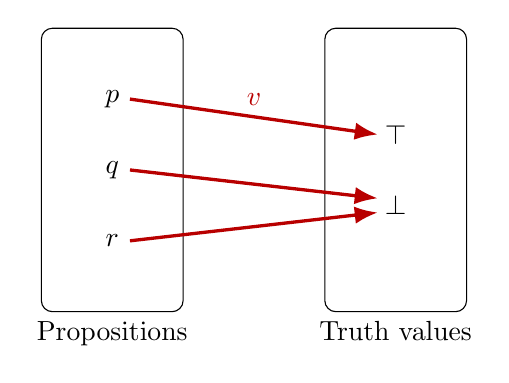
\begin{tikzpicture}[scale=0.9]
        \draw[rounded corners] (-3, 0) rectangle (-1, -4) {};
        \draw[rounded corners] (1, 0) rectangle (3, -4) {};

        \node[align=center, anchor=center] at (-2, -1) {\(p\)};
        \node[align=center, anchor=center] at (-2, -2) {\(q\)};
        \node[align=center, anchor=center] at (-2, -3) {\(r\)};

        \node[align=center, anchor=center] at (2, -1.5) {\(\top\)};
        \node[align=center, anchor=center] at (2, -2.5) {\(\bot\)};

        \draw[-Latex, very thick, BrickRed] (-1.75, -1) -- (1.75, -1.5) node[pos=0.5, anchor=south] {\(v\)};

        \draw[-Latex, very thick, BrickRed] (-1.75, -2) -- (1.75, -2.4);

        \draw[-Latex, very thick, BrickRed] (-1.75, -3) -- (1.75, -2.6);

        \node[anchor=north] at (-2, -4) {Propositions};

        \node[anchor=north] at (2, -4) {Truth values};
        
    \end{tikzpicture}
    \caption{A valuation maps propositions to truth values.}
    \label{fig:Ch01-valuation}
\end{figure}

A valuation \(v\) can be extended to a unique \emph{truth function} defined on all possible formulas. A truth function \(v'\) must satisfy
%
\begin{align*}
    v'(\neg \phi) = \top &\iff v'(\phi) = \bot\\
    v'(\phi \lor \psi) = \top &\iff v'(\phi) = \top \text{ or } v'(\psi) = \top\\
    v'(\phi \land \psi) = \top &\iff v'(\phi) = \top \text{ and } v'(\psi) = \top\\
    v'(\phi \rightarrow \psi) = \top &\iff v'(\phi) = \bot \text{ or } v'(\psi) = \top\\
    v'(\phi \leftrightarrow \psi) = \top &\iff v'(\phi) = v'(\psi)
\end{align*}
%
for all formulas \(\phi\) and \(\psi\). From now on we use \(v\) to denote the more general truth function.

The result of applying a valuation \(v\) to a formula \(\phi\) depends only on the propositional letters that occur in \(\phi\). 

A formula \(\phi\) is \emph{valid} if \(v(\phi) = \top\) for all valuations \(v\), which we denote as \(\models \phi\). A formula \(\phi\) is \emph{satisfiable} if \(v(\phi) = \top\) for at least one valuation \(v\). All valid formulas are satisfiable, but \emph{not} vice versa.

Two formulas \(\phi\) and \(\psi\) are \emph{logically equivalent}, written as \(\phi \equiv \psi\), if and only if for every valuation \(v\) we have \(v(\phi) = v(\psi)\).



\subsubsection{Truth tables}

Consider the propositional formula \(((p \lor \neg q) \land \neg (q \land r))\). We can check its validity and satisfiability by constructing its truth table.

\begin{table}[H]
    \centering
    \begin{tabular}{|c|c|c||c|c||c|}
        \hline
        \(p\) & \(q\) & \(r\) & \((p \lor \neg q)\) & \(\neg (q \land r)\) & \(((p \lor \neg q) \land \neg (q \land r))\)\\
        \hline
        0 & 0 & 0 & 1 & 1 & 1 \\
        \hline
        0 & 0 & 1 & 1 & 1 & 1 \\
        \hline
        0 & 1 & 0 & 0 & 1 & 0 \\
        \hline
        0 & 1 & 1 & 0 & 0 & 0\\
        \hline
        1 & 0 & 0 & 1 & 1 & 1 \\
        \hline
        1 & 0 & 1 & 1 & 1 & 1 \\
        \hline
        1 & 1 & 0 & 1 & 1 & 1 \\
        \hline
        1 & 1 & 1 & 1 & 0 & 0 \\
        \hline
    \end{tabular}

    \caption{The truth table for the formula \(((p \lor \neg q) \land \neg (q \land r))\).}
    \label{tab:Ch01-truth-table}
\end{table}

In this case, the formula is satisfiable but not valid.



\subsubsection{Parse trees}

A parser interprets the semantics of a formula by breaking down its symbols into a \emph{parse tree}, which shows the syntactic relation between symbols. For example, the formula \(((p \lor \neg q) \land \neg (q \land r))\) can be broken down into the following parse tree.

\begin{figure}[H]
    \centering
    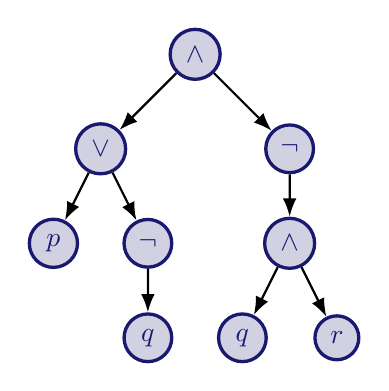
\begin{tikzpicture}[scale=0.6]
        \node (main-and) at (0,0)[circle, draw=MidnightBlue, very thick, MidnightBlue, fill=MidnightBlue!20] {\(\land\)};
        \node (or) at (-2,-2)[circle, draw=MidnightBlue, very thick, MidnightBlue, fill=MidnightBlue!20] {\(\lor\)};
        \node (right-neg) at (2,-2)[circle, draw=MidnightBlue, very thick, MidnightBlue, fill=MidnightBlue!20] {\(\neg\)};
        \node (p) at (-3,-4)[circle, draw=MidnightBlue, very thick, MidnightBlue, fill=MidnightBlue!20] {\(p\)};
        \node (left-neg) at (-1,-4)[circle, draw=MidnightBlue, very thick, MidnightBlue, fill=MidnightBlue!20] {\(\neg\)};
        \node (and) at (2,-4)[circle, draw=MidnightBlue, very thick, MidnightBlue, fill=MidnightBlue!20] {\(\land\)};
        \node (left-q) at (-1,-6)[circle, draw=MidnightBlue, very thick, MidnightBlue, fill=MidnightBlue!20] {\(q\)};
        \node (right-q) at (1,-6)[circle, draw=MidnightBlue, very thick, MidnightBlue, fill=MidnightBlue!20] {\(q\)};
        \node (r) at (3,-6)[circle, draw=MidnightBlue, very thick, MidnightBlue, fill=MidnightBlue!20] {\(r\)};

        \draw[-Latex, thick] (main-and) -- (or);
        \draw[-Latex, thick] (main-and) -- (right-neg);
        \draw[-Latex, thick] (or) -- (p);
        \draw[-Latex, thick] (or) -- (left-neg);
        \draw[-Latex, thick] (right-neg) -- (and);
        \draw[-Latex, thick] (left-neg) -- (left-q);
        \draw[-Latex, thick] (and) -- (right-q);
        \draw[-Latex, thick] (and) -- (r);
    \end{tikzpicture}
    \caption{The parse tree for the formula \(((p \lor \neg q) \land \neg (q \land r))\).}
    \label{fig:Ch01-parse-tree}
\end{figure}



\subsubsection{Disjunctive normal form (DNF)}

A formula is said to be in \emph{disjunctive normal form} (DNF) if it is a disjunction of one or more conjunctions of one or more literals.
%
\begin{align*}
    \text{proposition} &\coloneq p \;\vert\; q \;\vert\; r \;\vert\; \cdots\\
    \text{literal} &\coloneq \text{proposition} \;\vert\; \neg\text{proposition}\\
    \text{conjunctiveClause} &\coloneq \text{literal} \;\vert\; \text{literal } \land \text{ conjunctiveClause}\\
    \text{DNF} &\coloneq \text{conjunctiveClause} \;\vert\; \text{conjunctiveClause } \lor \text{ DNF}
\end{align*}
%
Below is an example of a formula in DNF.
%
\[
    {\color{BrickRed}\underbrace{(p \land \neg q \land \neg r)}_{\substack{\text{conjunctive}\\\text{clause}}}}
    \lor
    {\color{BrickRed}\underbrace{(\neg p \land \neg q \land r)}_{\substack{\text{conjunctive}\\\text{clause}}}}
    \lor
    {\color{BrickRed}\underbrace{(q \land \neg r)}_{\substack{\text{conjunctive}\\\text{clause}}}}
\]

Any propositional formula has a DNF equivalent. For instance, the formula \((p \lor \neg q) \land \neg (q \land r)\) can be rewritten as follows.
%
\begin{align*}
    & (p \lor \neg q) \land \neg (q \land r)\\
    \iff & (p \lor \neg q) \land (\neg q \lor \neg r) \tag{De Morgan's law, to remove outer negation}\\
    \iff & {\color{BrickRed}((p \lor \neg q) \land \neg q)} \lor {\color{MidnightBlue}((p \lor \neg q) \land \neg r)} \tag{distributing conjunctions over disjunctions}\\
    \iff & {\color{BrickRed}(p \land \neg q) \lor (\neg q \land \neg q)} \lor {\color{MidnightBlue}(p \land \neg r) \lor (\neg q \land \neg r)} \tag{distributing conjunctions over disjunctions}\\
    \iff & {\color{BrickRed}(p \land \neg q) \lor \neg q} \lor {\color{MidnightBlue}(p \land \neg r) \lor (\neg q \land \neg r)}
\end{align*}

Alternatively, this can also be achieved by referring to the truth table. From Table \ref{tab:Ch01-truth-table}, we see that the formula can be written in DNF as
%
\[(\neg p \land \neg q \land \neg r) \lor (\neg p \land \neg q \land r) \lor (p \land \neg q \land \neg r)  \lor (p \land \neg q \land r)  \lor (p \land q \land \neg r)\text{.}\]



\subsubsection{Conjunctive normal form (CNF)}

A formula is said to be \emph{conjunctive normal form} (CNF) if it is a conjunction of one or more disjunctions of one or more literals.
%
\begin{align*}
    \text{disjunctiveClause} &\coloneq \text{literal} \;\vert\; \text{literal } \lor \text{ disjunctiveClause}\\
    \text{CNF} &\coloneq \text{disjunctiveClause} \;\vert\; \text{disjunctiveClause } \land \text{ CNF}
\end{align*}
%
Below is a formula in CNF.
%
\[
    {\color{BrickRed}\underbrace{(p \lor \neg q \lor \neg r)}_{\substack{\text{conjunctive}\\\text{clause}}}}
    \land
    {\color{BrickRed}\underbrace{(\neg p \lor q \lor r)}_{\substack{\text{conjunctive}\\\text{clause}}}}
\]

To find the CNF equivalent of a formula \(\phi\), we first express its negation \(\neg\phi\) in DNF. Then, we negate it again to get \(\neg\neg\phi\). Using De Morgan's law, the resultant formula will be in CNF.

For example, let \(\phi\) be the formula \((p \lor \neg q) \land \neg (q \land r)\). To rewrite it in CNF, we start by constructing the truth table of its negation \(\neg\phi\). This allows us to express \(\neg\phi\) in DNF.

\begin{table}[H]
    \centering
    \begin{tabular}{|c|c|c||c|c|}
        \hline
        \(p\) & \(q\) & \(r\) & \(((p \lor \neg q) \land \neg (q \land r))\) & Negation of \(((p \lor \neg q) \land \neg (q \land r))\)\\
        \hline
        0 & 0 & 0 & 1 & 0 \\
        \hline
        0 & 0 & 1 & 1 & 0 \\
        \hline
        0 & 1 & 0 & 0 & 1 \\
        \hline
        0 & 1 & 1 & 0 & 1 \\
        \hline
        1 & 0 & 0 & 1 & 0 \\
        \hline
        1 & 0 & 1 & 1 & 0 \\
        \hline
        1 & 1 & 0 & 1 & 0 \\
        \hline
        1 & 1 & 1 & 0 & 1 \\
        \hline
    \end{tabular}

    \caption{The truth table for the negation of \(((p \lor \neg q) \land \neg (q \land r))\). This is obtained by flipping the results of Table \ref{tab:Ch01-truth-table}.}
    \label{tab:Ch01-truth-table-of-negation}
\end{table}

Hence we have
%
\begin{align*}
    \neg\phi &= (\neg p \land q) \lor (p \land q \land r) \tag{DNF of \(\neg\phi\)}\\
    \neg\neg\phi &= \neg((\neg p \land q) \lor (p \land q \land r)) \tag{negating both sides}\\
    \phi &= (p \lor \neg q) \land (\neg p \lor \neg q \lor \neg r) \tag{double negation; De Morgan's laws}
\end{align*}
%
which gives us \(\phi\) in CNF.



\subsection{First-order logic}

\subsubsection{Syntax}

A first-order language \(L(C, F, P)\) is determined by a set \(C\) of constant symbols, a set \(F\) of function symbols and a non-empty set \(P\) of predicate symbols. Each function symbol and predicate symbol has an associated \emph{arity} \(n \in \mathbb{N}\). We write \(f^n\) and \(p^n\) to represent an \(n\)-ary function symbol and an \(n\)-ary predicate symbol respectively. Moreover, let \(V\) be a countably infinite set of variable symbols.
%
\begin{align*}
    \text{term} &\coloneq c \;\vert\; v \;\vert\; f^n (\text{term}_0, \text{term}_1, \cdots, \text{term}_{n-1}) \tag{where \(c \in C\), \(v \in V\) and \(f^n \in F\)}\\
    \text{atom} &\coloneq p^n (\text{term}_0, \text{term}_1, \cdots, \text{term}_{n-1}) \tag{where \(p^n \in P\)}\\
    \text{formula} &\coloneq \text{atom} \;\vert\; \neg \text{formula} \;\vert\; (\text{formula}_0 \lor \text{formula}_1) \;\vert\; \exists v\; \text{formula}  \tag{where \(v \in V\)}
\end{align*}
%
This definition is functionally complete. Formulas involving universal quantifiers, implications and equivalence symbols can always be rewritten using only symbols defined above.

A \emph{closed term} is a term with no variable symbols. A \emph{sentence} is a formula with no free variables.



\subsubsection{Semantics}

For a first-order language \(L(C, F, P)\), we may construct a corresponding first-order structure\footnote{Also known as an \(L\)-structure.} \(S = (D, I)\) where \(I = (I_c, I_f, I_p)\).
%
{\large
    \[
        S = (
            {\color{BrickRed}
                \underbrace{D}_{\substack{
                    \text{non-empty}\\
                    \text{domain}
                }}
            }
            ,
            {\color{MidnightBlue}
                \overbrace{(
                    I_c,
                    I_f,
                    I_p
                )}^{\text{interpretation } I}
            }
        )
    \]
}
%
Here,
\begin{itemize}
    \item \(I_c\) maps each constant symbol in \(C\) to an element of \(D\).
    \item \(I_f\) maps each \(n\)-ary function symbol in \(F\) to an \(n\)-ary function over \(D\).
    \item \(I_p\) maps each \(n\)-ary predicate symbol \(p \in P\) to an \(n\)-ary relation over \(D\) (i.e. a subset of \(D^n\)).
    \item We may occasionally use \(I\) to denote a general interpretation function where
    %
    \begin{align*}
        I(c) &= I_c (c) \tag{for all \(c \in C\)}\\
        I(f) &= I_f (f) \tag{for all \(f \in F\)}\\
        I(p) &= I_p (p) \tag{for all \(p \in P\)}
    \end{align*}
\end{itemize}

If \(P\) includes the equality symbol \(=\), then it is always interpreted as the binary relation of true equality.
%
\[I_p (=) = \{(d, d) : d \in D\}\]

Given a structure \(S = (D, I)\), a variable assignment \(A\) is a map from \(V\) to \(D\). For any variable \(v \in V\), two variable assignments \(A\) and \(A^{*}\) are said to be \(v\)-equivalent if \(A(x) = A^{*}(x)\) for all \(x \in V \setminus \{v\}\). In other words, two variable assignments are said to be \(v\)-equivalent if they are completely identical except possibly for the element in \(D\) assigned to \(v\). This is written as \(A \equiv_v A^{*}\).

Given a structure \(S\) and a variable assignment \(A\), we may interpret any term as follows.
%
\begin{align*}
    c^{S, A} &= I_c (c)\\
    v^{S, A} &= A(v)\\
    f^n (t_0, t_1, \cdots, t_{n-1})^{S, A} &= {\color{MidnightBlue} \underbrace{(I_f (f^n))}_{\substack{\text{interpreted}\\\text{function}}}} (t_0^{S, A}, t_1^{S, A}, \cdots, t_{n-1}^{S, A})
\end{align*}

Formulas are evaluated as follows.
%
\begin{align*}
    S \models_A p^n (t_0, t_1, \cdots, t_{n-1}) &\iff (t_0^{S, A}, t_1^{S, A}, \cdots, t_{n-1}^{S, A}) \in I_p (p^n)\\
    S \models_A \neg \text{formula} &\iff S \not\models_A \text{formula}\\
    S \models_A (\text{formula}_0 \lor \text{formula}_1) &\iff S \models_A \text{formula}_0 \text{ or } S \models_A \text{formula}_1\\
    % S \models_A (\text{formula}_0 \land \text{formula}_1) &\iff S \models_A \text{formula}_0 \text{ and } S \models_A \text{formula}_1\\
    % S \models_A (\text{formula}_0 \rightarrow \text{formula}_1) &\iff S \not\models_A \text{formula}_0 \text{ or } S \models_A \text{formula}_1\\
    S \models_A \exists v\; \text{formula} &\iff S \models_{A[x \mapsto d]} \text{formula for some } d \in D
\end{align*}

Given a structure \(S\) and a formula \(\phi\), we say that
%
\begin{itemize}
    \item \(\phi\) is ``valid in \(S\)'' if \(S \models_A \phi\) for every variable assignment \(A\). This is written as \(S \models \phi\).
    \item \(\phi\) is ``satisfiable in \(S\)'' if \(S \models_A \phi\) for some variable assignment \(A\).
    \item \(\phi\) is ``valid'' if \(\phi\) is valid in all possible structures. This is written as \(\models \phi\).
    \item \(\phi\) is ``satisfiable'' if there exists some structure in which \(\phi\) is satisfiable.
\end{itemize}
%
A formula \(\phi\) is valid if and only if \(\neg \phi\) is not satisfiable.
%
\begin{quote}
    \textbf{Proof.} Let \(\neg\phi\) be a formula that is not satisfiable. Hence we have
    %
    \begin{align*}
        \neg \exists S\; \exists A\;\;\; S \models_A \neg\phi &\iff \neg \exists S\; \exists A\;\;\; S \not\models_A \phi\\
        &\iff \forall S\; \neg \exists A\;\;\; S \not\models_A \phi\\
        &\iff \forall S\; \forall A\;\;\;  \neg S \not\models_A \phi\\
        &\iff \forall S\; \forall A\;\;\; S \models_A \phi
    \end{align*}
    %
    which means \(S\) is valid.
\end{quote}

If \(\phi\) is a sentence, then \(\phi\) is valid in \(S\) if and only if it is also satisfiable in \(S\).



\subsubsection{Example: Arithmetic in the set of natural numbers}

Consider the first-order language \(L(C, F, P)\) defined as follows. Also assume a countably infinite set \(V\) of variable symbols.
%
\begin{align*}
    C &= 1, 2, 3, \cdots \tag{constant symbols}\\
    F &= \{+, \times\} \tag{function symbols, both binary}\\
    P &= \{=, <\} \tag{predicate symbols, both binary}\\
    V &= \{x, y, z, \cdots\} \tag{variable symbols}
\end{align*}
%
A term is a string of symbols that represents a ``thing'' or an ``object'' --- this can be a constant, a variable, or a function output.
%
\begin{itemize}
    \item \(x\)
    \item \(1 + 3\)
    \item \(2 \times x + 1\)
\end{itemize}
%
Of the terms shown above, only the second one is a closed terms because it has no variable symbols.

An atom is a string of symbols that represents the output of a predicate, which is a truth value.
%
\begin{itemize}
    \item \(1 = 2\)
    \item \(y < 3\)
    \item \(x + 1 < 2 \times z + 3\)
\end{itemize}
%
Finally, a formula is constructed by applying negations, disjunctions, and existential quantifiers to atoms.
%
\begin{itemize}
    \item \(1 = 2 \;\land\; y < 3\)
    \item \(\neg \exists z\;\; x + 1 < 2 \times z + 3\)
\end{itemize}
%
The latter example is a sentence because all of its variable symbols are bounded.

For this particular first-order language, we may use the structure of ordinary arithmetic\footnote{There is also a similar structure \(R = (\mathbb{R}, I)\) where the domain is the set of real numbers.}, defined as \(N = \{\mathbb{N}, \{I_c, I_f, I_p\}\}\) where
%
\begin{itemize}
    \item \(I_c\) is a function that maps numerical symbols to the corresponding natural number.
    %
    \begin{align*}
        I_c (1) &= 1\\
        I_c (2) &= 2\\
        I_c (3) &= 3\\
        &\;\;\vdots
    \end{align*}

    \item \(I_f\) maps \(+\) and \(\times\) to the addition and multiplication operations in arithmetic respectively.
    
    \item \(I_p\) maps \(=\) and \(<\) to the following relations.
    %
    \begin{align*}
        I_p (=) &= \{(n, n) : n \in \mathbb{N}\}\\
        I_p (<) &= \{(m, n) \in \mathbb{N}^2 : m < n\}
    \end{align*}
\end{itemize}



\subsubsection{First-order structures and directed graphs}

Consider a first-order language with only one binary predicate symbol \(p\).
%
\[L(C, F, {\color{BrickRed} \{p\}})\]
%
Any first-order structure \(S = \{D, \{I_c, I_f, I_p\}\}\) for this language can be represented as a directed graph, where each vertex is an element of \(D\) and each directed edge represents an element of the relation \(I_p (p)\).

\begin{figure}[H]
    \centering
    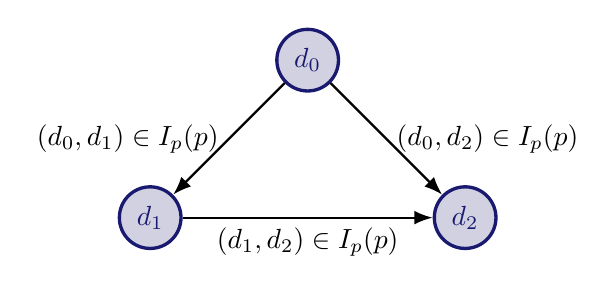
\begin{tikzpicture}
        \node (d0) at (0,0)[circle, draw=MidnightBlue, very thick, MidnightBlue, fill=MidnightBlue!20] {\(d_0\)};
        \node (d1) at (-2,-2)[circle, draw=MidnightBlue, very thick, MidnightBlue, fill=MidnightBlue!20] {\(d_1\)};
        \node (d2) at (2,-2)[circle, draw=MidnightBlue, very thick, MidnightBlue, fill=MidnightBlue!20] {\(d_2\)};

        \draw[-Latex, thick] (d0) -- (d1) node[pos=0.5, left]{\((d_0, d_1) \in I_p (p)\)};

        \draw[-Latex, thick] (d0) -- (d2) node[pos=0.5, right]{\((d_0, d_2) \in I_p (p)\)};

        \draw[-Latex, thick] (d1) -- (d2) node[pos=0.5, below]{\((d_1, d_2) \in I_p (p)\)};
        
    \end{tikzpicture}
    \caption{The first-order structure \(S\) can be visualised as a directed graph.}
    \label{fig:Ch01-first-order-structure-as-directed-graph}
\end{figure}

\newpage
\section{Axiomatic Proofs for Propositional Logic}

A \emph{proof system} is a system for determining the validity of formulas.

An obvious system would be to construct a truth table and check that all rows give a true result. However, this naive approach has an exponential time complexity\footnote{Using this system, checking the validity of a formula with \(n\) proposition symbols requires \(2^n\) computations.}, meaning that it will become increasingly impractical as more and more propositions are introduced. To alleviate this issue, we will introduce a different approach below.



\subsection{Axiomatic proof system}

Firstly, we limit our propositional language to only use the connectives \(\neg\) and \(\rightarrow\). Double negations are prohibited.

Moreover, we will note some \emph{axioms} that are known to be valid, and then try to derive other valid formulas from the axioms. Below we list three different \emph{schemas}, from which axioms may be obtained by substituting any formulas in place of \(p\), \(q\) and \(r\).
%
\begin{enumerate}[I.]
    \item \(p \rightarrow (q \rightarrow p)\)
    \item \((p \rightarrow (q \rightarrow r)) \rightarrow ((p \rightarrow q) \rightarrow (p \rightarrow r))\)
    \item \((\neg p \rightarrow \neg q) \rightarrow (q \rightarrow p)\)
\end{enumerate}

Axioms on their own are insufficient in establishing a proof system. We also need \emph{inference rules}, which stipulate how conclusions can be derived from premises. One of the main inference rules is \emph{modus ponens}, which states that if you have proved both the formula \(\phi\) and the implication \((\phi\rightarrow\psi)\), then you may deduce the conclusion \(\psi\).
%
\[
    \infer{\psi}{
        \phi
        &
        (\phi\rightarrow\psi)
    }
    %
    \tag{modus ponens}
\]

In this system, a \emph{proof} is a sequence of formulas
%
\[\phi_0,\; \phi_1,\; \phi_2,\; \cdots \phi_n\]
%
such that for each \(i \leq n\), the formula \(\phi_i\) is either
%
\begin{itemize}
    \item an axiom; or
    \item obtained from two previous formulas \(\phi_j\) and \(\phi_k\) in the sequence via modus ponens (for some \(j, k < i\)).
\end{itemize}
%
If such a proof exists, then the final formula \(\phi_n\) is called a \emph{theorem} and we may write \(\vdash \phi_n\).

\begin{figure}[H]
    \centering
    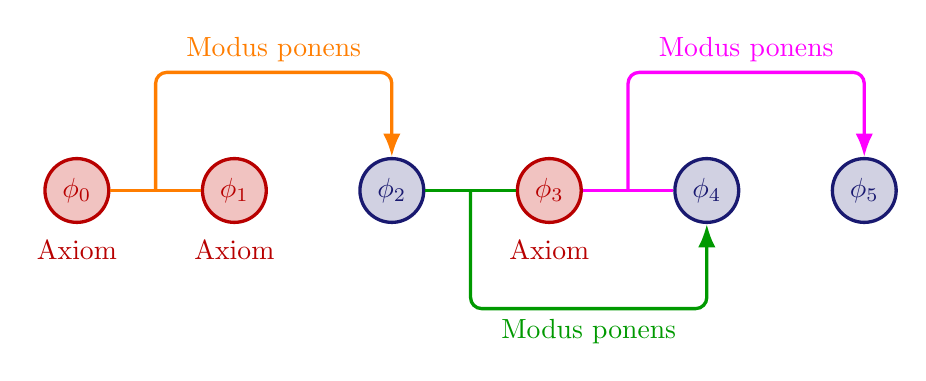
\begin{tikzpicture}
        \foreach \i in {0,1,3} {
            \node (\i) at (2*\i, 0)[circle, draw=BrickRed, very thick, BrickRed, fill=BrickRed!20] {\(\phi_\i\)};

            \draw node[yshift=-0.75cm, BrickRed] at (2*\i, 0) {Axiom};
        }

        \foreach \i in {2,4,5} {
            \node (\i) at (2*\i, 0)[circle, draw=MidnightBlue, very thick, MidnightBlue, fill=MidnightBlue!20] {\(\phi_\i\)};
        }

        \draw[BurntOrange, very thick] (0) -- (1);
        \draw[BurntOrange, very thick, -Latex, rounded corners] (1, 0) -- (1, 1.5) -- (4,1.5) node[pos=0.5, above]{Modus ponens} -- (2);
        
        \draw[OliveGreen, very thick] (2) -- (3);
        \draw[OliveGreen, very thick, -Latex, rounded corners] (5, 0) -- (5, -1.5) -- (8,-1.5) node[pos=0.5, below]{Modus ponens} -- (4);
        
        \draw[Fuchsia, very thick] (3) -- (4);
        \draw[Fuchsia, very thick, -Latex, rounded corners] (7, 0) -- (7, 1.5) -- (10,1.5) node[pos=0.5, above]{Modus ponens} -- (5);
    \end{tikzpicture}
    \caption{In a proof, every formula must be either an axiom, or derived from previous formulas via modus ponens.}
    \label{fig:Ch02-proof}
\end{figure}



\newpage
\section{Propositional tableau}

In view of the impracticality of Hilbert-style proof systems, we introduce below an easier and more implementable method for determining a formula's validity --- \emph{tableaus}.

Here is a brief overview of how a tableau works. Suppose we want to check the satisfiability of a formula \(\phi\). This formula will be placed at the root of a binary tree, called a tableau. We use a variety of expansion rules to grow the tree until it is complete. An \emph{open} tableau indicates that \(\phi\) is satisfiable, while a \emph{closed} tableau indicates that \(\phi\) is unsatisfiable.

To determine the validity of a formula, simply construct a tableau for \(\neg\phi\). If the resultant tableau is open, then \(\neg\phi\) is satisfiable, so \(\phi\) is invalid. On the contrary, if the resultant tableau is closed, then \(\neg\phi\) must be unsatisfiable, so \(\phi\) is valid.


\subsection{Constructing a tableau}

In a tableau, every node is marked with a formula. To build a tableau for a formula \(\phi\), begin by placing \(\phi\) at the root of a binary tree. Then, we repeat the following process:
%
\begin{enumerate}
    \item Select a formula in the tree that has not been selected before. The formula must not be a literal.
    \item Choose the expansion rule (see below) that applies to the selected formula.
    \item For each leaf node, add new children nodes in accordance to the chosen expansion rule.
    \item Place a tick beside the selected formula to make sure we don't expand it again.
\end{enumerate}

There are two types of expansion rules:
%
\begin{itemize}
    \item \(\alpha\)-rules, which create one new child per leaf node; and
    \item \(\beta\)-rules, which create two new children per leaf node.
\end{itemize}

Figures \ref{fig:Ch03-alpha-rules} and \ref{fig:Ch03-beta-rules} depict the \(\alpha\)- and \(\beta\) rules respectively. Nodes that are newly created by each rule are highlighted in blue.


\begin{figure}[H]
    \centering
    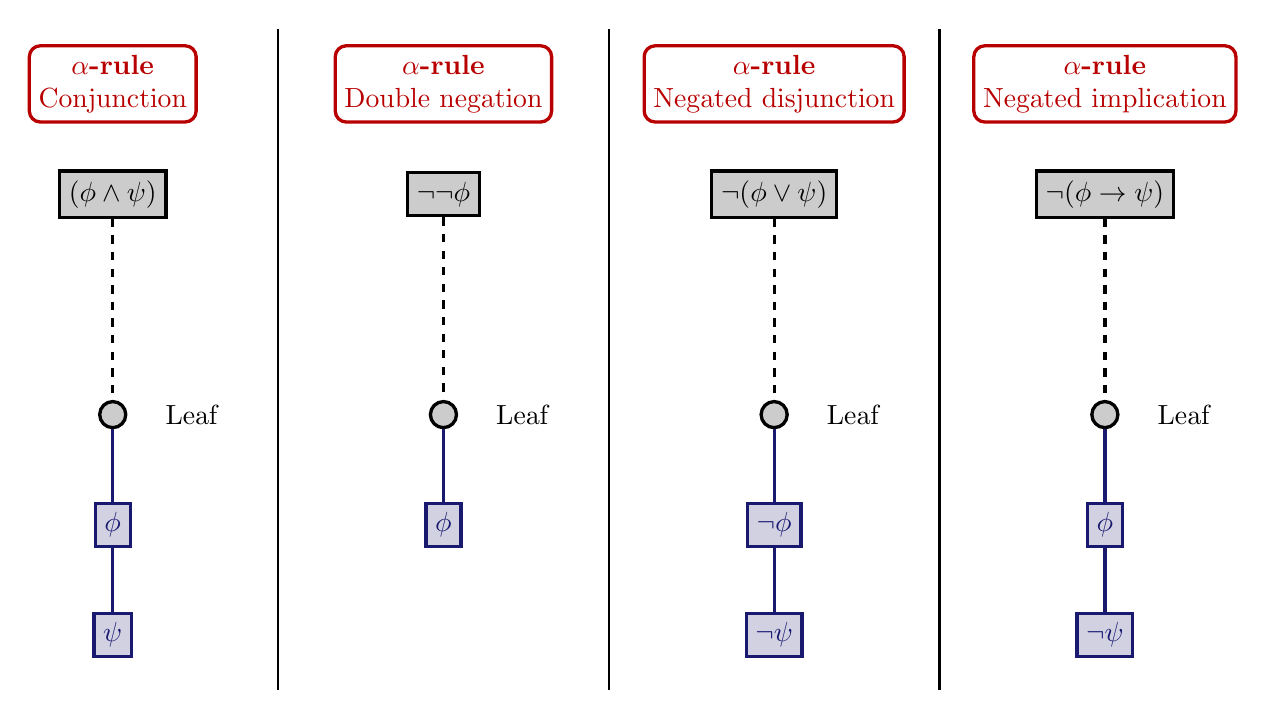
\begin{tikzpicture}[scale=1.4]
        \begin{scope}[shift={(0, 0)}]
            \node (root) at (0, 1)[draw=BrickRed, very thick, BrickRed, rounded corners, align=center] {\textbf{\(\alpha\)-rule} \\ Conjunction};

            \node (root) at (0, 0)[draw=black, very thick, fill=black!20] {\((\phi\land\psi)\)};

            \node (leaf) at (0, -2)[circle, draw=black, very thick, fill=black!20] {};

            \node [right of=leaf, black] {Leaf};

            \draw[dashed, very thick] (root) -- (leaf);

            \node (child1) at (0, -3)[draw=MidnightBlue, very thick, MidnightBlue, fill=MidnightBlue!20] {\(\phi\)};

            \node (child2) at (0, -4)[draw=MidnightBlue, very thick, MidnightBlue, fill=MidnightBlue!20] {\(\psi\)};

            \draw[very thick, MidnightBlue] (leaf) -- (child1) -- (child2);
        \end{scope}

        \begin{scope}[shift={(3, 0)}]
            \node (root) at (0, 1)[draw=BrickRed, very thick, BrickRed, rounded corners, align=center] {\textbf{\(\alpha\)-rule} \\ Double negation};

            \node (root) at (0, 0)[draw=black, very thick, fill=black!20] {\(\neg\neg\phi\)};

            \node (leaf) at (0, -2)[circle, draw=black, very thick, fill=black!20] {};

            \node [right of=leaf, black] {Leaf};

            \draw[dashed, very thick] (root) -- (leaf);

            \node (child1) at (0, -3)[draw=MidnightBlue, very thick, MidnightBlue, fill=MidnightBlue!20] {\(\phi\)};

            \draw[very thick, MidnightBlue] (leaf) -- (child1);
        \end{scope}

        \begin{scope}[shift={(6, 0)}]
            \node (root) at (0, 1)[draw=BrickRed, very thick, BrickRed, rounded corners, align=center] {\textbf{\(\alpha\)-rule} \\ Negated disjunction};

            \node (root) at (0, 0)[draw=black, very thick, fill=black!20] {\(\neg(\phi\lor\psi)\)};

            \node (leaf) at (0, -2)[circle, draw=black, very thick, fill=black!20] {};

            \node [right of=leaf, black] {Leaf};

            \draw[dashed, very thick] (root) -- (leaf);

            \node (child1) at (0, -3)[draw=MidnightBlue, very thick, MidnightBlue, fill=MidnightBlue!20] {\(\neg\phi\)};

            \node (child2) at (0, -4)[draw=MidnightBlue, very thick, MidnightBlue, fill=MidnightBlue!20] {\(\neg\psi\)};

            \draw[very thick, MidnightBlue] (leaf) -- (child1) -- (child2);
        \end{scope}

        \begin{scope}[shift={(9, 0)}]
            \node (root) at (0, 1)[draw=BrickRed, very thick, BrickRed, rounded corners, align=center] {\textbf{\(\alpha\)-rule} \\ Negated implication};

            \node (root) at (0, 0)[draw=black, very thick, fill=black!20] {\(\neg(\phi\rightarrow\psi)\)};

            \node (leaf) at (0, -2)[circle, draw=black, very thick, fill=black!20] {};

            \node [right of=leaf, black] {Leaf};

            \draw[dashed, very thick] (root) -- (leaf);

            \node (child1) at (0, -3)[draw=MidnightBlue, very thick, MidnightBlue, fill=MidnightBlue!20] {\(\phi\)};

            \node (child2) at (0, -4)[draw=MidnightBlue, very thick, MidnightBlue, fill=MidnightBlue!20] {\(\neg\psi\)};

            \draw[very thick, MidnightBlue] (leaf) -- (child1) -- (child2);
        \end{scope}
        
        \foreach \x in {1.5, 4.5, 7.5} {
            \draw[thick] (\x, 1.5) -- (\x, -4.5);
        }
    \end{tikzpicture}
    \caption{The four \(\alpha\)-rules for constructing propositional tableaus.}
    \label{fig:Ch03-alpha-rules}
\end{figure}


\begin{figure}[H]
    \centering
    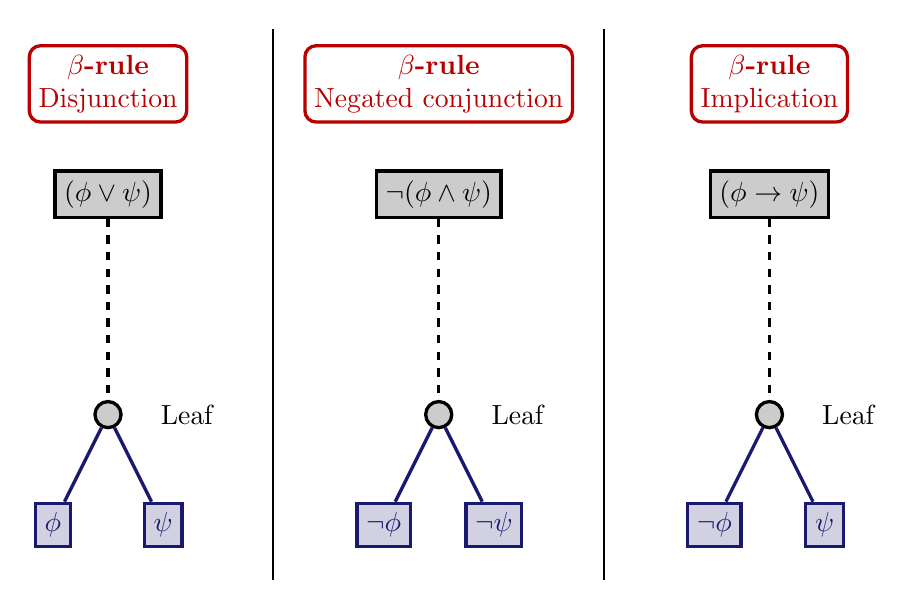
\begin{tikzpicture}[scale=1.4]
        \begin{scope}[shift={(0, 0)}]
            \node (root) at (0, 1)[draw=BrickRed, very thick, BrickRed, rounded corners, align=center] {\textbf{\(\beta\)-rule} \\ Disjunction};

            \node (root) at (0, 0)[draw=black, very thick, fill=black!20] {\((\phi\lor\psi)\)};

            \node (leaf) at (0, -2)[circle, draw=black, very thick, fill=black!20] {};

            \node [right of=leaf, black] {Leaf};

            \draw[dashed, very thick] (root) -- (leaf);

            \node (child1) at (-0.5, -3)[draw=MidnightBlue, very thick, MidnightBlue, fill=MidnightBlue!20] {\(\phi\)};

            \node (child2) at (0.5, -3)[draw=MidnightBlue, very thick, MidnightBlue, fill=MidnightBlue!20] {\(\psi\)};

            \draw[very thick, MidnightBlue] (leaf) -- (child1);
            \draw[very thick, MidnightBlue] (leaf) -- (child2);
        \end{scope}

        \begin{scope}[shift={(3, 0)}]
            \node (root) at (0, 1)[draw=BrickRed, very thick, BrickRed, rounded corners, align=center] {\textbf{\(\beta\)-rule} \\ Negated conjunction};

            \node (root) at (0, 0)[draw=black, very thick, fill=black!20] {\(\neg(\phi\land\psi)\)};

            \node (leaf) at (0, -2)[circle, draw=black, very thick, fill=black!20] {};

            \node [right of=leaf, black] {Leaf};

            \draw[dashed, very thick] (root) -- (leaf);

            \node (child1) at (-0.5, -3)[draw=MidnightBlue, very thick, MidnightBlue, fill=MidnightBlue!20] {\(\neg\phi\)};

            \node (child2) at (0.5, -3)[draw=MidnightBlue, very thick, MidnightBlue, fill=MidnightBlue!20] {\(\neg\psi\)};

            \draw[very thick, MidnightBlue] (leaf) -- (child1);
            \draw[very thick, MidnightBlue] (leaf) -- (child2);
        \end{scope}

        \begin{scope}[shift={(6, 0)}]
            \node (root) at (0, 1)[draw=BrickRed, very thick, BrickRed, rounded corners, align=center] {\textbf{\(\beta\)-rule} \\ Implication};

            \node (root) at (0, 0)[draw=black, very thick, fill=black!20] {\((\phi\rightarrow\psi)\)};

            \node (leaf) at (0, -2)[circle, draw=black, very thick, fill=black!20] {};

            \node [right of=leaf, black] {Leaf};

            \draw[dashed, very thick] (root) -- (leaf);

            \node (child1) at (-0.5, -3)[draw=MidnightBlue, very thick, MidnightBlue, fill=MidnightBlue!20] {\(\neg\phi\)};

            \node (child2) at (0.5, -3)[draw=MidnightBlue, very thick, MidnightBlue, fill=MidnightBlue!20] {\(\psi\)};

            \draw[very thick, MidnightBlue] (leaf) -- (child1);
            \draw[very thick, MidnightBlue] (leaf) -- (child2);
        \end{scope}
        
        \foreach \x in {1.5, 4.5} {
            \draw[thick] (\x, 1.5) -- (\x, -3.5);
        }
    \end{tikzpicture}
    \caption{The three \(\beta\)-rules for constructing propositional tableaus.}
    \label{fig:Ch03-beta-rules}
\end{figure}

In general, nodes located in the same branch\footnote{A \emph{branch} is defined as a path from the root of the tableau to one of its leaves.} are considered in conjunction while the different branches are considered to be disjuncted. As a result, a tableau is a tree-like representation of a formula that is a disjunction of conjunctions, à la disjunctive normal form (DNF).

A tableau is considered \emph{complete} if every node is either ticked (already expanded) or a literal. When a tableau is complete, we can determine the original formula's satisfiability as follows.
%
\begin{itemize}
    \item A branch containing both a propositional letter and its negation (\(p\) and \(\neg p\)) is said to be \emph{closed}, which we denote as \(\oplus\). Otherwise, it is \emph{open}.
    \item A tableau where all branches are closed is said to be \emph{closed}, meaning that the formula at its root is unsatisfiable. Contrarily, a tableau with at least one open branch is said to be \emph{open}, indicating that the formula is satisfiable.
\end{itemize}



\subsection{Example of constructing a tableau and converting to DNF}

To check if the formula
%
\[((p \lor q) \land (\neg p \rightarrow \neg q))\]
%
is satisfiable, we construct its tableau, as shown in figure \ref{fig:Ch03-satisfiability-tableau}.

Since only one of the four branches is closed, this formula is satisfiable. In fact, the literals in each open branch give a possible valuation that satisfies the given formula. For instance, the second branch from the left contains the literals \(p\) and \(\neg q\). This indicates that the formula is true when \(p\) is true and \(q\) is false.

\begin{figure}[H]
    \centering
    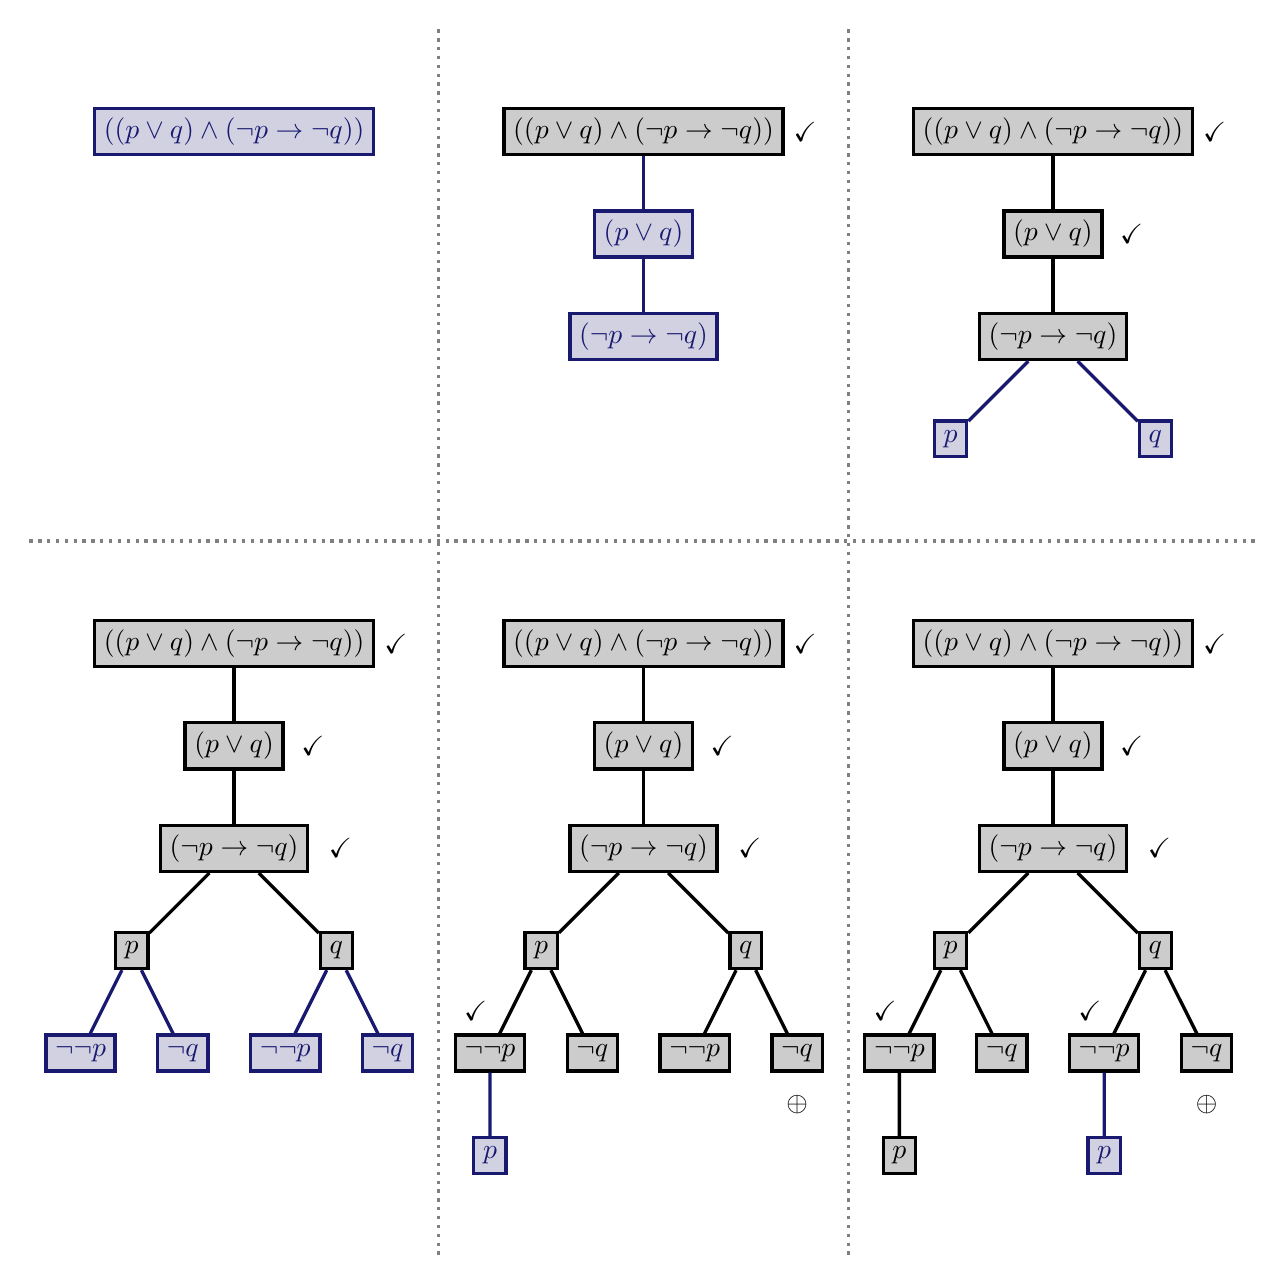
\begin{tikzpicture}[scale=1.3]
        \begin{scope}[shift={(0, 0)}]
            \node (0) at (0, 0)[draw=MidnightBlue, very thick, MidnightBlue, fill=MidnightBlue!20] {\(((p \lor q) \land (\neg p \rightarrow \neg q))\)};
        \end{scope}

        \begin{scope}[shift={(4, 0)}]
            \node (0) at (0, 0)[draw=black, very thick, fill=black!20] {\(((p \lor q) \land (\neg p \rightarrow \neg q))\)};
            \node[right of=0, xshift=30pt] {\checkmark};

            \node (1) at (0, -1)[draw=MidnightBlue, very thick, MidnightBlue, fill=MidnightBlue!20] {\((p \lor q)\)};

            \node (2) at (0, -2)[draw=MidnightBlue, very thick, MidnightBlue, fill=MidnightBlue!20] {\((\neg p \rightarrow \neg q)\)};

            \draw[MidnightBlue, very thick] (0) -- (1) -- (2);
        \end{scope}

        \begin{scope}[shift={(8, 0)}]
            \node (0) at (0, 0)[draw=black, very thick, fill=black!20] {\(((p \lor q) \land (\neg p \rightarrow \neg q))\)};
            \node[right of=0, xshift=30pt] {\checkmark};

            \node (1) at (0, -1)[draw=black, very thick, fill=black!20] {\((p \lor q)\)};
            \node[right of=1] {\checkmark};

            \node (2) at (0, -2)[draw=black, very thick, fill=black!20] {\((\neg p \rightarrow \neg q)\)};

            \node (3) at (-1, -3)[draw=MidnightBlue, very thick, MidnightBlue, fill=MidnightBlue!20] {\(p\)};

            \node (4) at (1, -3)[draw=MidnightBlue, very thick, MidnightBlue, fill=MidnightBlue!20] {\(q\)};

            \draw[black, very thick] (0) -- (1) -- (2);
            \draw[MidnightBlue, very thick] (2) -- (3);
            \draw[MidnightBlue, very thick] (2) -- (4);
        \end{scope}

        \begin{scope}[shift={(0, -5)}]
            \node (0) at (0, 0)[draw=black, very thick, fill=black!20] {\(((p \lor q) \land (\neg p \rightarrow \neg q))\)};
            \node[right of=0, xshift=30pt] {\checkmark};

            \node (1) at (0, -1)[draw=black, very thick, fill=black!20] {\((p \lor q)\)};
            \node[right of=1] {\checkmark};

            \node (2) at (0, -2)[draw=black, very thick, fill=black!20] {\((\neg p \rightarrow \neg q)\)};
            \node[right of=2, xshift=10pt] {\checkmark};

            \node (3) at (-1, -3)[draw=black, very thick, fill=black!20] {\(p\)};

            \node (4) at (1, -3)[draw=black, very thick, fill=black!20] {\(q\)};

            \node (5) at (-1.5, -4)[draw=MidnightBlue, very thick, MidnightBlue, fill=MidnightBlue!20] {\(\neg\neg p\)};

            \node (6) at (-0.5, -4)[draw=MidnightBlue, very thick, MidnightBlue, fill=MidnightBlue!20] {\(\neg q\)};

            \node (7) at (0.5, -4)[draw=MidnightBlue, very thick, MidnightBlue, fill=MidnightBlue!20] {\(\neg\neg p\)};

            \node (8) at (1.5, -4)[draw=MidnightBlue, very thick, MidnightBlue, fill=MidnightBlue!20] {\(\neg q\)};

            \draw[black, very thick] (0) -- (1) -- (2);
            \draw[black, very thick] (2) -- (3);
            \draw[black, very thick] (2) -- (4);
            \draw[MidnightBlue, very thick] (3) -- (5);
            \draw[MidnightBlue, very thick] (3) -- (6);
            \draw[MidnightBlue, very thick] (4) -- (7);
            \draw[MidnightBlue, very thick] (4) -- (8);
        \end{scope}

        \begin{scope}[shift={(4, -5)}]
            \node (0) at (0, 0)[draw=black, very thick, fill=black!20] {\(((p \lor q) \land (\neg p \rightarrow \neg q))\)};
            \node[right of=0, xshift=30pt] {\checkmark};

            \node (1) at (0, -1)[draw=black, very thick, fill=black!20] {\((p \lor q)\)};
            \node[right of=1] {\checkmark};

            \node (2) at (0, -2)[draw=black, very thick, fill=black!20] {\((\neg p \rightarrow \neg q)\)};
            \node[right of=2, xshift=10pt] {\checkmark};

            \node (3) at (-1, -3)[draw=black, very thick, fill=black!20] {\(p\)};

            \node (4) at (1, -3)[draw=black, very thick, fill=black!20] {\(q\)};

            \node (5) at (-1.5, -4)[draw=black, very thick, fill=black!20] {\(\neg\neg p\)};
            \node[above left of=5, xshift=15pt, yshift=-5pt] {\checkmark};

            \node (6) at (-0.5, -4)[draw=black, very thick, fill=black!20] {\(\neg q\)};

            \node (7) at (0.5, -4)[draw=black, very thick, fill=black!20] {\(\neg\neg p\)};

            \node (8) at (1.5, -4)[draw=black, very thick, fill=black!20] {\(\neg q\)};
            \node [below of=8, yshift=10pt] {\(\oplus\)};
            
            \node (9) at (-1.5, -5)[draw=MidnightBlue, very thick, MidnightBlue, fill=MidnightBlue!20] {\(p\)};

            \draw[black, very thick] (0) -- (1) -- (2);
            \draw[black, very thick] (2) -- (3);
            \draw[black, very thick] (2) -- (4);
            \draw[black, very thick] (3) -- (5);
            \draw[black, very thick] (3) -- (6);
            \draw[black, very thick] (4) -- (7);
            \draw[black, very thick] (4) -- (8);
            \draw[MidnightBlue, very thick] (5) -- (9);
        \end{scope}

        \begin{scope}[shift={(8, -5)}]
            \node (0) at (0, 0)[draw=black, very thick, fill=black!20] {\(((p \lor q) \land (\neg p \rightarrow \neg q))\)};
            \node[right of=0, xshift=30pt] {\checkmark};

            \node (1) at (0, -1)[draw=black, very thick, fill=black!20] {\((p \lor q)\)};
            \node[right of=1] {\checkmark};

            \node (2) at (0, -2)[draw=black, very thick, fill=black!20] {\((\neg p \rightarrow \neg q)\)};
            \node[right of=2, xshift=10pt] {\checkmark};

            \node (3) at (-1, -3)[draw=black, very thick, fill=black!20] {\(p\)};

            \node (4) at (1, -3)[draw=black, very thick, fill=black!20] {\(q\)};

            \node (5) at (-1.5, -4)[draw=black, very thick, fill=black!20] {\(\neg\neg p\)};
            \node[above left of=5, xshift=15pt, yshift=-5pt] {\checkmark};

            \node (6) at (-0.5, -4)[draw=black, very thick, fill=black!20] {\(\neg q\)};

            \node (7) at (0.5, -4)[draw=black, very thick, fill=black!20] {\(\neg\neg p\)};
            \node[above left of=7, xshift=15pt, yshift=-5pt] {\checkmark};

            \node (8) at (1.5, -4)[draw=black, very thick, fill=black!20] {\(\neg q\)};
            \node [below of=8, yshift=10pt] {\(\oplus\)};
            
            \node (9) at (-1.5, -5)[draw=black, very thick, fill=black!20] {\(p\)};

            \node (10) at (0.5, -5)[draw=MidnightBlue, very thick, MidnightBlue, fill=MidnightBlue!20] {\(p\)};

            \draw[black, very thick] (0) -- (1) -- (2);
            \draw[black, very thick] (2) -- (3);
            \draw[black, very thick] (2) -- (4);
            \draw[black, very thick] (3) -- (5);
            \draw[black, very thick] (3) -- (6);
            \draw[black, very thick] (4) -- (7);
            \draw[black, very thick] (4) -- (8);
            \draw[black, very thick] (5) -- (9);
            \draw[MidnightBlue, very thick] (7) -- (10);
        \end{scope}

        \draw[gray, very thick, dotted] (2, 1) -- (2, -11);
        \draw[gray, very thick, dotted] (6, 1) -- (6, -11);
        \draw[gray, very thick, dotted] (-2, -4) -- (10, -4);
    \end{tikzpicture}
    \caption{Constructing the tableau of \(((p \lor q) \land (\neg p \rightarrow \neg q))\). Read from left to right and from top to bottom.}
    \label{fig:Ch03-satisfiability-tableau}
\end{figure}

It follows that given the tableau of a formula, its DNF equivalent can be expressed as
%
\[
    \smashoperator{
        \mathop{
            \mathlarger{\mathlarger{\mathlarger{
                \lor
            }}}
        }
    }_{\text{open branch } \Theta}
    \left(
        \mathlarger{\mathlarger{\mathlarger{
            \land
        }}}
        \;\raisebox{2pt}{\(\{\text{literals in } \Theta\}\)}
    \right)
    \text{.}
\]

As always, the CNF of a formula can be obtained by negating the DNF form of its negation.

\end{document}